\pattern{Proxy}
\begin{summary}
    A {\bf proxy} is a wrapper or agent object that is being called by the
    client or user to access the real object behind the scenes.

    This pattern is widely used in applications that require security
    protection and access control.
\end{summary}

\subsubsection{Implementation details}
In general, a proxy is a class that is functioning as an interface (or
placeholder) to something else. 
\begin{description}
    \item[Virtual Proxy (a type of caching)] Proxy returns a default or cached
        result if the real object either takes some time to create or involves
        heavy computation. Virtual proxies delay the initialization or 
        computation of the real object until it is needed.
    \item[Remote Proxy] Used when a resource is remote. Communicating with the
        real object might involve serialization or marshalling of data. That
        logic is encapsulated in these proxies. 
    \item[Protection Proxy] Used for access control and partial encapsulation.
        Users will only have access to functions provided by the interface. 
        The application provides different interfaces to different clients with
        different access rights.
\end{description}

\comparison{\begin{itemize}
        \item Maintainability: Internal change to the ``Real Subject'' does
            not affect the proxy consumers because access is abstracted through 
            the proxy interface.  Developers can easily add new methods into
            the interface for clients to use.
        \item Low Coupling: reduces the coupling between client and the real
            subject by providing an abstracted interface between the client
            and subject.
        \item Performance: The use of caching in the proxy can increase
            the performance of some systems.
    \end{itemize}
}{\begin{itemize}
        \item Performance: The extra layer of abstraction could impact 
            performance in some cases.
    \end{itemize}
}% END comparison

\begin{nfps}
\item[Security] Proxy pattern guarantees that only authorized users can access
    the resource. Different interfaces can be seen as different access rights.
\item[Performance] The initialization of expensive objects can be delayed by
    using a proxy object that exposes the same interface as the original 
    object. Caching and delayed initialization allow for performance gains.
\item[Negative Inconsistency] ``This pattern introduces another layer of
    abstraction which sometimes may be an issue if the {\sc RealSubject} code
    is accessed by some of the clients directly and some of them might access
    the {\sc Proxy} classes. This might cause disparate behaviour.'' 
\item[Negative Ambiguity] The client may not know that the {\sc RealSubject} it
    is accessing now is not same as the previous one.
\end{nfps}

\subsubsection{Example}
Proxies are often used to interface with a network connection, a large object
in memory, a file, or some other resource that involves heavy computation or
that is impossible to duplicate.

The banking application below with deposit functions is an example.

\begin{center}
    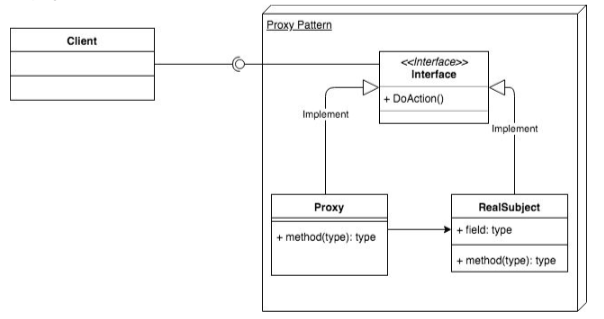
\includegraphics[width=0.4\textwidth]{./proxy1}
    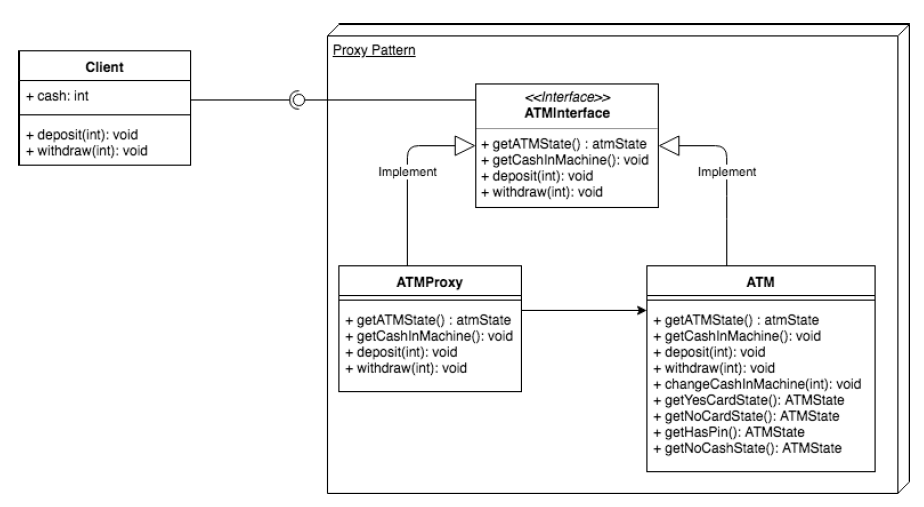
\includegraphics[width=0.4\textwidth]{./proxy2}
\end{center}

